% ===== CHAPTER 6 =====
\chapter{氢原子}
\label{chap:6}
    
\section{单粒子中心力问题}
\label{sec:6.1 The One-Particle Central Force Problem}
    在研究氢原子之前,我们先来看看单个粒子在中心力作用下运动这一更为普遍的问题。本节的结果适用于任何中心力问题。例如氢原子(第 \ref{sec:6.5 The Hydrogen Atom} 节)和各向同性的三维谐振子(第 \ref{sec:6.3 Reduction of the Two-Particle Problem to Two One-Particle Problems} 节)。

    \textbf{中心力}(central force)是由球面对称的势能函数导出的,这意味着中心力只是粒子与原点距离的函数$V = V\left(r\right)$。力和势能的关系由式(\ref{eq:5.31})给出:
    \begin{equation}
        F - \nabla V\left(x,y,z\right) = -\mathbf{i}\left(\partial V/\partial x\right) - \mathbf{j}\left(\partial V/\partial y\right) - \mathbf{k}\left(\partial V/\partial z\right)
        \label{eq:6.1}
    \end{equation}
    (\ref{eq:6.1})中的偏导数可以用链式法则求得[式(\ref{eq:5.53})- \ref{eq:5.55}]。在这个例子中,由于$V$只是$r$的函数,所以我们有$\left(\partial V/\partial\theta\right)_{r,\phi} = 0$和$\left(\partial V/\partial\phi\right)_{r,\theta} = 0$。因此,
    \begin{equation}
        \left(\frac{\partial V}{\partial x}\right)_{y,z} = \frac{\mathrm{d}V}{\mathrm{d}r}\left(\frac{\partial r}{\partial x}\right)_{y,z} = \frac{x}{r}\frac{\mathrm{d}V}{\mathrm{d}r}
        \label{eq:6.2}
    \end{equation}
    \begin{equation}
        \left(\frac{\partial V}{\partial y}\right)_{x,z} = \frac{y}{r}\frac{\mathrm{d}V}{\mathrm{d}r}, \quad \left(\frac{\partial V}{\partial z}\right)_{x,y} = \frac{z}{r}\frac{\mathrm{d}V}{\mathrm{d}r}
        \label{eq:6.3}
    \end{equation}
    其中我们用到了式(\ref{eq:5.57})和(\ref{eq:5.58})。则方程(\ref{eq:6.1})可以写成
    \begin{equation}
        \mathbf{F} = -\frac{1}{r}\frac{\mathrm{d}V}{\mathrm{d}r}\left(x\mathbf{i}+y\mathbf{j}+z\mathbf{k}\right) = -\frac{\mathrm{d}V\left(r\right)}{\mathrm{d}r}\frac{\mathbf{r}}{r}
        \label{eq:6.4}
    \end{equation}
    其中$\mathbf{r}$的计算使用了式(\ref{eq:5.33})。式(\ref{eq:6.4})中的$\mathbf{r}/r$是径向上的单位矢量。因此中心力是径向的。

    现在,让我们来看看受中心力作用的单粒子量子力学。其哈密顿算符为
    \begin{equation}
        \hat{H} = \hat{T} + \hat{V} = -\left(\hbar^2/2m\right)\nabla^2 + V\left(r\right)
        \label{eq:6.5}
    \end{equation}
    其中$\nabla^2 \equiv \partial^2/\partial x^2 + \partial^2/\partial y^2 + \partial^2/\partial z^2$[式(\ref{eq:3.46})]。由于$V$是球对称的,我们将在球坐标系中进行计算。因此,我们希望将拉普拉斯算符转换为球坐标的形式。我们已经有了$\partial/\partial x$、$\partial/\partial y$和$\partial /\partial z$的表达式[式(\ref{eq:5.62})-(\ref{eq:5.65})],通过将这些算符平方并相加,我们就得到了拉普拉斯算符。该计算留作课后习题。结果为(问题6.4):
    \begin{equation}
        \nabla^2 = \frac{\partial^2}{\partial r^2} + \frac{2}{r}\frac{\partial}{\partial r} + \frac{1}{r^2}\frac{\partial^2}{\partial\theta^2} + \frac{1}{r^2}\cot\theta\frac{\partial}{\partial\theta} + \frac{1}{r^2\sin^2\theta}\frac{\partial^2}{\partial\phi^2}
        \label{eq:6.6}
    \end{equation}

    回过头来看式(\ref{eq:5.68}),其中给出了单粒子轨道角动量大小平方的算符$\hat{L}^2$,我们可以看到
    \begin{equation}
        \nabla^2 = \frac{\partial^2}{\partial r^2} + \frac{2}{r}\frac{\partial}{\partial r} - \frac{1}{r^2\hbar^2}\hat{L}^2
        \label{eq:6.7}
    \end{equation}
    哈密顿算符(\ref{eq:6.5})变为
    \begin{equation}
        \hat{H} = -\frac{\hbar^2}{2m}\left(\frac{\partial^2}{\partial r^2} + \frac{2}{r}\frac{\partial}{\partial r}\right) + \frac{1}{2mr^2}\hat{L}^2 + V\left(r\right)
        \label{eq:6.8}
    \end{equation}

    在经典力学中,受中心力作用的粒子其角动量是守恒的(第\ref{sec:5.3 Angular Momentum of a One-Particle System}节)。在量子力学中,我们可能会问,我们是否可以拥有能量和角动量都有确定值的状态?为了使$\hat{H}$的本征函数组也是$\hat{L}^2$的本征函数,对易子$\left[\hat{H},\hat{L}^2\right]$必须为零。我们有
    \begin{equation*}
        \left[\hat{H},\hat{L}^2\right] = \left[\hat{T},\hat{L}^2\right] + \left[\hat{V},\hat{L}^2\right]
    \end{equation*}
    \begin{equation*}
        \left[\hat{T}, \hat{L}^2\right] = \left[-\frac{\hbar^2}{2m}\left(\frac{\partial ^2}{\partial r^2} + \frac{2}{r}\frac{\partial}{\partial r}\right) + \frac{1}{2mr^2}\hat{L}^2, \hat{L}^2\right]
    \end{equation*}
    \begin{equation}
        \left[\hat{T},\hat{L}^2\right] = -\frac{\hbar^2}{2m}\left[\frac{\partial^2}{\partial r^2} + \frac{2}{r}\frac{\partial}{\partial r}, \hat{L}^2\right] + \frac{1}{2m}\left[\frac{1}{r^2}\hat{L}^2, \hat{L}^2\right]
        \label{eq:6.9}
    \end{equation}
    回忆$\hat{L}^2$只是$\theta$和$\phi$的函数,而不是$r$的函数[式(\ref{eq:5.68})]。因此它与任何包含$r$的算符可对易。[为了证明这一结论,我们必须使用(\ref{eq:5.47})类似的关系,但将$x$和$z$分别换成$r$和$\theta$。]因此,式(\ref{eq:6.9})中第一项的对易子为零。此外,由于任何算符都与它自己对易,式(\ref{eq:6.9})第二项的对易子也为零。因此,$\left[\hat{T},\hat{L}^2\right] = 0$。同样地,由于$\hat{L}^2$不包含$r$,$V$只是$r$的函数,我们有$\left[\hat{V},\hat{L}^2\right] = 0$。因此,
    \begin{equation}
        \left[\hat{H},\hat{L}^2\right] = 0, \quad \text{若} V = V\left(r\right)
        \label{eq:6.10}
    \end{equation}
    当势能函数与$\theta$和$\phi$都无关时,$\hat{H}$和$\hat{L}^2$可对易。

    现在,我们来考虑算符$\hat{L}_z = -\mathrm{i}\hbar\partial/\partial\phi$[式(\ref{eq:5.67})]。由于$\hat{L}_z$不包含$r$,因此它与$\hat{L}^2$可对易[式(\ref{eq:5.50})],因此$\hat{H}$(\ref{eq:6.8})和$\hat{L}_z$也可对易。我们有
    \begin{equation}
        \left[\hat{H}, \hat{L}_z\right] = 0, \quad \text{若} V = V\left(r\right)
        \label{eq:6.11}
    \end{equation}

    因此,我们现在有了中心力问题中,一组同时是$\hat{H}$、$\hat{L}^2$和$\hat{L}_z$的本征函数的函数。令$\psi$表示这些共同本征函数:
    \begin{equation}
        \boxed{
            \hat{H}\psi = E\psi
        }
        \label{eq:6.12}
    \end{equation}
    \begin{equation}
        \boxed{
            \hat{L}^2\psi = l\left(l+1\right)\hbar^2\psi, \quad l = 0, 1, 2, \ldots
        }
        \label{eq:6.13}
    \end{equation}
    \begin{equation}
        \boxed{
            \hat{L}_z\psi = m\hbar\psi, \quad m = -l, -l+1, \ldots, l-1, l
        }
        \label{eq:6.14}
    \end{equation}
    其中,我们用到了式(\ref{eq:5.104})和式(\ref{eq:5.105})。

    根据式(\ref{eq:6.8})和(\ref{eq:6.13}),对薛定谔方程(\ref{eq:6.12}),有
    \begin{equation*}
        -\frac{\hbar^2}{2m}\left(\frac{\partial^2}{\partial r^2} + \frac{2}{r}\frac{\partial}{\partial r}\right) + \frac{1}{2mr^2}\hat{L}^2\psi + V\left(r\right)\psi = E\psi
    \end{equation*}
    \begin{equation}
        -\frac{\hbar^2}{2m}\left(\frac{\partial^2}{\partial r^2} + \frac{2}{r}\frac{\partial}{\partial r}\right) + \frac{l\left(l+1\right)\hbar^2}{2mr^2}\psi + V\left(r\right)\psi = E\psi
        \label{eq:6.15}
    \end{equation}

    $\hat{L}^2$的本征函数是球谐函数$Y_l^m\left(\theta, \phi\right)$,由于$\hat{L}^2$不包含$r$,我们可以将任意一个关于$r$的函数与球谐函数相乘,新函数依然是$\hat{L}^2$和$\hat{L}_z$的本征函数。因此,
    \begin{equation}
        \boxed{
            \psi = R\left(r\right)Y_l^m\left(\theta, \phi\right)
        }
        \label{eq:6.16}
    \end{equation}
    将(\ref{eq:6.16})代入(\ref{eq:6.15}),然后两边同除以$Y_l^m$,得到关于未知函数$R\left(r\right)$的微分方程:
    \begin{equation}
        -\frac{\hbar^2}{2m}\left(R^{\prime\prime}+ \frac{2}{r}R^{\prime}\right) + \frac{l\left(l+1\right)\hbar^2}{2mr^2}R + V\left(r\right)R = ER\left(r\right)
        \label{eq:6.17}
    \end{equation}

    我们已经证明:\textit{对于任意势能函数$V\left(r\right)$是球对称的单粒子问题,定态波函数为$\psi = R\left(r\right)Y_l^m\left(\theta, \phi\right)$,其中$R\left(r\right)$满足微分方程(\ref{eq:6.17})。}通过指定式(\ref{eq:6.17})中势能函数$V\left(r\right)$的形式,我们可以针对某个特定问题解决它。

\section{非相互作用粒子和变量分离}
\label{sec:6.2 Noninteracting Particles and Separation of Variables}
    到目前为止,我们只解决了单粒子量子力学问题。氢原子是一个双粒子系统,作为处理氢原子的第一步,我们首先考虑一个更简单的情况,即两个不相互作用的粒子。

    假设一个系统由两个无相互作用的粒子1和2组成。令$q_1$和$q_2$分别表示粒子1的$\left(x_1,y_1,z_1\right)$坐标和粒子2的$\left(x_2,y_2,z_2\right)$坐标。由于粒子之间没有相互作用力,系统的经典机械能就是两个粒子的能量之和:$E = E_1+E_2 = T_1+V_1 + T_2 + V_2$,经典哈密顿量是两个粒子哈密顿量之和:$H = H_1 + H_2$。因此,系统的哈密顿算符为
    \begin{equation*}
        \hat{H} = \hat{H}_1 + \hat{H}_2
    \end{equation*}
    其中$\hat{H}_1$只和坐标$q_1$有关,动量算符$\hat{p}_1$对应于$q_1$。系统的薛定谔方程为
    \begin{equation}
        \left(\hat{H}_1 + \hat{H}_2\right)\psi\left(q_1,q_2\right) = E\psi\left(q_1,q_2\right)
        \label{eq:6.18}
    \end{equation}
    我们尝试用分离变量法来求解(\ref{eq:6.18}),令
    \begin{equation}
        \psi\left(q_1,q_2\right) = G_1\left(q_1\right)G_2\left(q_2\right)
        \label{eq:6.19}
    \end{equation}
    我们有
    \begin{equation}
        \hat{H}_1G_1\left(q_1\right)G_2\left(q_2\right) + \hat{H}_2G_1\left(q_1\right)G_2\left(q_2\right) = EG_1\left(q_1\right)G_2\left(q_2\right)
        \label{eq:6.20}
    \end{equation}
    由于$\hat{H}_1$只包含粒子1的位置和动量算符,我们有$\hat{H}_1\left[G_1\left(q_1\right)G_2\left(q_2\right)\right] = G_2\left(q_2\right)\hat{H}_1G_1\left(q_1\right)$,因此,就$\hat{H}_1$而言,$G_2\left(q_2\right)$是常数。使用这个方程以及类似的关于$\hat{H}_2$的方程,我们发现(\ref{eq:6.20})变为
    \begin{equation}
        G_2\left(q_2\right)\hat{H}_1G_1\left(q_1\right) + G_1\left(q_1\right)\hat{H}_2G_2\left(q_2\right) = EG_1\left(q_1\right)G_2\left(q_2\right)
        \label{eq:6.21}
    \end{equation}
    \begin{equation}
        \frac{\hat{H}_1G_1\left(q_1\right)}{G_1\left(q_1\right)} + \frac{\hat{H}_2G_2\left(q_2\right)}{G_2\left(q_2\right)} = E
        \label{eq:6.22}
    \end{equation}
    现在,通过与式 (\ref{eq:3.65}) 相同的论证,我们得出结论:在 (\ref{eq:6.22}) 中,左边的每项必须是常数。令$E_1$和$E_2$分别表示这些常数,我们有
    \begin{equation*}
        \frac{\hat{H}_1G_1\left(q_1\right)}{G_1\left(q_1\right)} = E_1, \quad \frac{\hat{H}_2G_2\left(q_2\right)}{G_2\left(q_2\right)} = E_2
    \end{equation*}
    \begin{equation}
        E = E_1 + E_2
        \label{eq:6.23}
    \end{equation}
    因此,当系统由两个无相互作用的粒子组成时,通过求解下式,我们可以将双粒子问题简化为两个单粒子问题:
    \begin{equation}
        \hat{H}_1G_1\left(q_1\right) = E_1G_1\left(q_1\right), \quad \hat{H}_2G_2\left(q_2\right) = E_2G_2\left(q_2\right)
        \label{eq:6.24}
    \end{equation}
    它们是每个粒子的独立薛定谔方程。

    将该结果推广到$n$个无相互作用的粒子,我们有
    \begin{equation*}
        \hat{H} = \hat{H}_1 + \hat{H}_2 + \ldots + \hat{H}_n
    \end{equation*}
    \begin{equation}
        \boxed{
                \psi\left(q_1,q_2,\ldots,q_n\right) = G_1\left(q_1\right)G_2\left(q_2\right)\ldots G_n\left(q_n\right)
        }
        \label{eq:6.25}
    \end{equation}
    \begin{equation}
        \boxed{
            E = E_1 + E_2 + \ldots + E_n
        }
        \label{eq:6.26}
    \end{equation}
    \begin{equation}
        \boxed{
            \hat{H}_iG_i = E_iG_i, \quad i = 1, 2, \ldots, n
        }
        \label{eq:6.27}
    \end{equation}
    \textit{对于一个无相互作用粒子系统,能量是每个粒子各自能量的总和,波函数是每个粒子波函数的乘积。利用哈密顿算符$\hat{H}_i$,求解粒子$i$的薛定谔方程,即可求得粒子$i$的波函数$G_i$。}

    这些结果也适用于单个粒子,其哈密顿算符是每个坐标的独立项之和:
    \begin{equation*}
        \hat{H} = \hat{H}_x\left(\hat{x},\hat{p}_x\right) + \hat{H}_y\left(\hat{y},\hat{p}_y\right) + \hat{H}_z\left(\hat{z},\hat{p}_z\right)
    \end{equation*}
    在这种情况下,我们得出结论:波函数和能量分别为
    \begin{equation*}
        \psi\left(x,y,z\right) = F\left(x\right)G\left(y\right)K\left(z\right), E = E_x + E_y + E_z
    \end{equation*}
    \begin{equation*}
        \hat{H}_xF\left(x\right) = E_xF\left(x\right), \quad \hat{H}_yG\left(y\right) = E_yG\left(y\right), \quad \hat{H}_zK\left(z\right) = E_zK\left(z\right)
    \end{equation*}
    例如三维盒子中的质点(第 \ref{sec:3.5 The Particle in a Three-Dimensional Box} 节)、三维自由质点(问题 3.42)和三维谐振子(问题 4.20)。
\section{将双粒子问题简化为两个单粒子问题}
\label{sec:6.3 Reduction of the Two-Particle Problem to Two One-Particle Problems}
    氢原子包含两个粒子——质子和电子。对于一个双粒子系统(粒子1的坐标为$\left(x_1,y_1,z_1\right)$,粒子2的坐标为$\left(x_2,y_2,z_2\right)$),粒子间相互作用的势能通常只是粒子相对坐标$x_2-x_1$、$y_2-y_1$和$z_2-z_1$的函数。在这种情况中,双粒子问题可以简化为两个单粒子问题,正如我们现在所要证明的。

    先考虑经典力学处理两个相互作用粒子的情况,令其质量分别为$m_1$和$m_2$。我们用从直角坐标系原点出发的半径矢量$\mathbf{r}_1$和$\mathbf{r}_2$来指定它们的位置(图\ref{fig:6.1})。粒子1和2的坐标分别为$\left(x_1,y_1,z_1\right)$和$\left(x_2,y_2,z_2\right)$。我们从粒子1到粒子2画出矢量$\mathbf{r} = \mathbf{r}_2 - \mathbf{r}_1$,并用$x$、$y$和$z$表示其分量:
    \begin{figure}[h!]
        \centering
        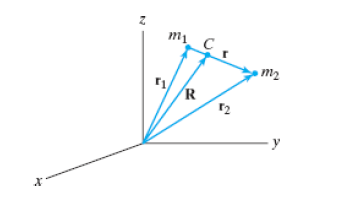
\includegraphics[width=0.4\textwidth]{Figures/6.1.png}
        \caption{质心位于$C$的双粒子系统}
        \label{fig:6.1}
    \end{figure}
    \begin{equation}
        \boxed{
            x = x_2 - x_1, \quad y = y_2 - y_1, \quad z = z_2 - z_1
        }
        \label{eq:6.28}
    \end{equation}
    $x$、$y$和$z$称为\textbf{相对坐标}或\textbf{内坐标}(relative or internal coordinates)。

    我们现在从原点指向系统的质心$C$画出矢量$\mathbf{R}$,其分量用$X$、$Y$和$Z$表示:
    \begin{equation}
        \mathbf{R} = \mathbf{i}X + \mathbf{j}Y + \mathbf{k}Z
        \label{eq:6.29}
    \end{equation}
    根据双粒子系统质心的定义,有
    \begin{equation}
        X = \frac{m_1x_1 + m_2x_2}{m_1 + m_2}, \quad Y = \frac{m_1y_1 + m_2y_2}{m_1 + m_2}, \quad Z = \frac{m_1z_1 + m_2z_2}{m_1 + m_2}
        \label{eq:6.30}
    \end{equation}
    这三个方程与矢量方程等价:
    \begin{equation}
        \mathbf{R} = \frac{m_1\mathbf{r}_1 + m_2\mathbf{r}_2}{m_1 + m_2}
        \label{eq:6.31}
    \end{equation}
    我们也有
    \begin{equation}
        \mathbf{r} = \mathbf{r}_2 - \mathbf{r}_1
        \label{eq:6.32}
    \end{equation}
    我们将式(\ref{eq:6.31})和(\ref{eq:6.32})联立为关于$\mathbf{r}_1$和$\mathbf{r}_2$的方程组,并求解得到
    \begin{equation}
        \mathbf{r}_1 = \mathbf{R} - \frac{m_2}{m_1 + m_2}\mathbf{r}, \quad \mathbf{r}_2 = \mathbf{R} + \frac{m_1}{m_1 + m_2}\mathbf{r}
        \label{eq:6.33}
    \end{equation}
    方程(\ref{eq:6.31})和(\ref{eq:6.32})代表了一种将$x_1,y_1,z_1$和$x_2,y_2,z_2$坐标转换为$X,Y,Z$和$x,y,z$坐标的变换。考虑一下在这种变化下,系统的哈密顿量会发生什么变化。用字母顶上的点表示对时间的导数。粒子1的速度为[式(\ref{eq:5.34})]$\mathbf{v}_1 = \mathrm{d}\mathbf{r}_1/\mathrm{d}t = \dot{\mathbf{r}}_1$。系统的动能为两个粒子的动能之和:
    \begin{equation}
        T = \frac{1}{2}m_1\left|\dot{\mathbf{r}_1}\right|^2 + \frac{1}{2}m_2\left|\dot{\mathbf{r}_2}\right|^2
        \label{eq:6.34}
    \end{equation}
    将(\ref{eq:6.33})的时间导数代入(\ref{eq:6.34}),我们得到
    \begin{equation*}
        \begin{aligned}
            T = & \frac{1}{2}m_1\left(\dot{\mathbf{R}} - \frac{m_2}{m_1+m_2}\dot{\mathbf{r}}\right)\cdot \left(\dot{\mathbf{R}} - \frac{m_2}{m_1+m_2}\dot{\mathbf{r}}\right) \\
            & + \frac{1}{2}m_2\left(\dot{\mathbf{R}} + \frac{m_1}{m_1+m_2}\dot{\mathbf{r}}\right)\cdot \left(\dot{\mathbf{R}} + \frac{m_1}{m_1+m_2}\dot{\mathbf{r}}\right) \\
        \end{aligned}
    \end{equation*}
    其中,我们用到了$\left|\mathbf{A}\right|^2 = \mathbf{A}\cdot \mathbf{A}$[式(\ref{eq:5.24})]。使用矢量数量积的分配律,化简后,我们得到
    \begin{equation}
        T = \frac{1}{2}\left(m_1 + m_2\right)\left|\dot{\mathbf{R}}\right|^2 + \frac{1}{2}\left(\frac{m_1m_2}{m_1+m_2}\right)\left|\dot{\mathbf{r}}\right|^2
        \label{eq:6.35}
    \end{equation}
    令$M$为系统的总质量:
    \begin{equation}
        M \equiv m_1 + m_2
        \label{eq:6.36}
    \end{equation}
    我们定义双粒子系统的\textbf{折合质量}(reduced mass)为
    \begin{equation}
        \boxed{
            \mu \equiv \frac{m_1m_2}{m_1+m_2}
        }
        \label{eq:6.37}
    \end{equation}
    那么
    \begin{equation}
        T = \frac{1}{2}M\left|\dot{\mathbf{R}}\right|^2 + \frac{1}{2}\mu\left|\dot{\mathbf{r}}\right|^2
        \label{eq:6.38}
    \end{equation}

    (\ref{eq:6.38})的第一项是质量为$M$的整个系统平动产生的动能。\textbf{平动}(translational motion)是指每个质点都经历相同位移的运动。$\frac{1}{2}M\left|\dot{\mathbf{R}}\right|^2$是位于质心,具有质量$M$的假想粒子的动能。(\ref{eq:6.38})的第二项是两个粒子内运动(相对运动)产生的动能。内运动有两种形式。两个粒子间的距离$r$可以变化(振动),以及矢量$\mathbf{r}$的方向可以发生变化(转动)。注意:$\left|\dot{\mathbf{r}}\right| = \left|\mathrm{d}\mathbf{r}/\mathrm{d}t\right| \neq \mathrm{d}\left|\mathbf{r}\right|/\mathrm{d}t$。

    与六个原始坐标$x_1,y_1,z_1,x_2,y_2,z_2$相对应,我们有六个线性动量:
    \begin{equation}
        p_{x_1} = m_1\dot{x}_1, \quad \ldots, \quad p_{z_2} = m_2\dot{z}_2
        \label{eq:6.39}
    \end{equation}
    将(\ref{eq:6.34})和(\ref{eq:6.38})相比较,我们将新坐标$X,Y,Z,x,y,z$的动量定义为
    \begin{equation*}
        p_X \equiv M\dot{X}, \quad p_Y \equiv M\dot{Y}, \quad p_Z \equiv M\dot{Z}
    \end{equation*}
    \begin{equation*}
        p_x \equiv \mu\dot{x}, \quad p_y \equiv \mu\dot{y}, \quad p_z \equiv \mu\dot{z}
    \end{equation*}
    我们定义两个新动量矢量:
    \begin{equation*}
        \mathbf{p}_M = \mathbf{i}M\dot{X} + \mathbf{j}M\dot{Y} + \mathbf{k}M\dot{Z},
        \quad \text{和} \quad \mathbf{p}_{\mu} = \mathbf{i}\mu\dot{x} + \mathbf{j}\mu\dot{y} + \mathbf{k}\mu\dot{z}
    \end{equation*}
    将这些动量代入式(\ref{eq:6.38}),我们得到
    \begin{equation}
        T = \frac{\left|\mathbf{p}_M\right|^2}{2M} + \frac{\left|\mathbf{p}_{\mu}\right|^2}{2\mu}
        \label{eq:6.40}
    \end{equation}

    现在,我们来考虑势能。我们限制$V$只是两个粒子的相对坐标$x$、$y$和$z$的函数:
    \begin{equation}
        V = V\left(x,y,z\right)
        \label{eq:6.41}
    \end{equation}
    (\ref{eq:6.41})的一个例子是相互作用遵守库仑定律的两个带电粒子[见式(\ref{eq:3.53})]。根据对$V$的这一限制,哈密顿函数为
    \begin{equation}
        H = \frac{p_M^2}{2M} + \left[\frac{p_{\mu}^2}{2\mu} + V\left(x,y,z\right)\right]
        \label{eq:6.42}
    \end{equation}

    现在,假设我们有一个由质量为 $M$ 的粒子和质量为 $\mu$ 的粒子组成的系统,前者不受力,后者受势能函数 $V\left(x,y,z\right)$ 的作用。再假设这些粒子之间没有相互作用。如果$\left(X,Y,Z\right)$表示质量为$M$的粒子的坐标,而$\left(x,y,z\right)$表示质量为$\mu$的粒子的坐标,那么这个假设系统的哈密顿量是什么?显然,它与式(\ref{eq:6.42})完全相同。

    哈密顿量(\ref{eq:6.42})可以看作是两个无相互作用假想粒子的哈密顿量之和:质量为$M$的粒子其哈密顿量为$p_M^2/2M$,质量为$\mu$的粒子其哈密顿量为$p_{\mu}^2/2\mu + V\left(x,y,z\right)$。因此,第\ref{sec:6.2 Noninteracting Particles and Separation of Variables}的结果表明:系统的量子力学能量是两个假想粒子的能量之和[式(\ref{eq:6.23})]:$E = E_M + E_{\mu}$。由式(\ref{eq:6.24})和(\ref{eq:6.42})可知,平动能$E_M$可以通过求解薛定谔方程$\left(\hat{p}_M^2/2M\right)\psi_M = E_M\psi_M$得到。这是质量为$M$的自由粒子的薛定谔方程,因此其可能的本征值全是非负数[式(\ref{neq:2.31})]:$E_m \ge 0$。由式(\ref{eq:6.42})和(\ref{eq:6.24})可知,内运动能$E_{\mu}$可以通过求解以下薛定谔方程得到:
    \begin{equation}
        \left[\frac{\hat{p}_{\mu}^2}{2\mu} + V\left(x,y,z\right)\right]\psi_{\mu}\left(x,y,z\right) = E_{\mu}\psi_{\mu}\left(x,y,z\right)
        \label{eq:6.43}
    \end{equation}

    这样,我们就把两个粒子根据仅取决于相对坐标 $x$、$y$、$z$ 的势能函数 $V\left(x,y,z\right)$ 进行相互作用的问题分离成了两个独立的单粒子问题:(1)质量为$M$的整体系统平动,它只是在系统能量的基础上增加了一个恒非负的能量$E_M$;(2)通过求解质量为 $\mu$ 的假想粒子的薛定谔方程 (\ref{eq:6.43})来处理相对运动或内部运动,该粒子的坐标为相对坐标 $x$、$y$、$z$,并在势能 $V\left(x,y,z\right)$ 的作用下运动。

    例如,对于包含一个电子(e)和一个质子(p)的氢原子,原子的总能量为$E = E_M + E_{\mu}$,其中的$E_M$是质量为$M = m_e+m_p$的整个原子在空间中的平动能,其中的$E_{\mu}$是通过将$\mu = m_em_p/(m_e+m_p)$代入(\ref{eq:6.43})得到的,$V$ 是电子和质子相互作用的库仑定律势能;见第 \ref{sec:6.5 The Hydrogen Atom} 节。

\section{双粒子的刚性转子模型}
\label{sec:6.4 The Two-Particle Rigid Rotor}
    在求解氢原子的薛定谔方程之前,我们先来处理双粒子的刚性转子。这是一个双粒子系统,粒子之间的距离固定,由一根长度为$d$的刚性无质量杆连接。对于这个问题,图\ref{fig:6.1}中的矢量$\mathbf{r}$的长度$\left|\mathbf{r}\right|$是常数$d$。因此(见第\ref{sec:6.3 Reduction of the Two-Particle Problem to Two One-Particle Problems}节),内运动的动能完全是转动能。转子的能量完全由动能提供,以及
    \begin{equation}
        V=0
        \label{eq:6.44}
    \end{equation}
    方程(\ref{eq:6.44})是(\ref{eq:6.41})的一个特例,因此,我们可以利用上一节得到的结果,将系统的平动分离出来。我们将只关注转动能量。旋转运动的哈密顿算符由(\ref{eq:6.43})中括号内的项给出:
    \begin{equation}
        \hat{H} = \frac{\hat{p}_{\mu}^2}{2\mu} = -\frac{\hbar^2}{2\mu}\nabla^2, \quad \mu = \frac{m_1m_2}{m_1+m_2}
        \label{eq:6.45}
    \end{equation}
    其中$m_1$和$m_2$是两个粒子的质量。质量为$\mu$的假想粒子的坐标为$m_1$和$m_2$之间的相对坐标。[式(\ref{eq:6.28})]。

    与使用相对笛卡尔坐标$x$、$y$和$z$不同,使用相对球坐标$r$、$\theta$和$\phi$来描述转子会更有成效。$r$坐标与图\ref{fig:6.1}中的矢量$\mathbf{r}$的长度相同,由于$m_1$和$m_2$受限于保持固定的距离,我们有$r=d$。因此,这个问题等价于一个质量为$\mu$的粒子受限在半径为$r$的球面上运动。由于径向坐标是恒定的,波函数将只是$\theta$和$\phi$的函数。因此,对波函数进行运算时,式(\ref{eq:6.8})中拉普拉斯算符的前两项为零,可以省略。换个角度看问题,我们注意到式(\ref{eq:6.8})中涉及$r$导数的算符对应于径向运动的动能,而由于没有径向运动,$\hat{H}$中不包含$r$的导数。

    由于$V=0$是$V=V\left(r\right)$的特例,第\ref{sec:6.1 The One-Particle Central Force Problem}节的结论表明:本征函数由式(\ref{eq:6.16})给出,其中$r$的因子被省略:
    \begin{equation}
        \psi = Y_l^m\left(\theta, \phi\right)
        \label{eq:6.46}
    \end{equation}
    其中,转动角量子数用$J$而不是$l$来表示。

    哈密顿算符由式(\ref{eq:6.8})给出,其中省略了$r$的导数及$V\left(r\right) = 0$。因此,
    \begin{equation*}
        \hat{H} = \left(2\mu d^2\right)^{-1}\hat{L}^2
    \end{equation*}
    使用式(\ref{eq:6.13}),有
    \begin{equation*}
        \begin{aligned}
            \hat{H}\psi & = E\psi \\
            \left(2\mu d^2\right)^{-1}\hat{L}^2Y_J^m\left(\theta, \phi\right) & = EY_J^m\left(\theta, \phi\right) \\
            \left(2\mu d^2\right)^{-1}J\left(J+1\right)\hbar^2Y_J^m\left(\theta, \phi\right) & = EY_J^m\left(\theta, \phi\right) \\
        \end{aligned}
    \end{equation*}
    \begin{equation}
        E = \frac{J\left(J+1\right)\hbar^2}{2\mu d^2}
        \label{eq:6.47}
    \end{equation}

    由$n$个粒子组成的系统绕空间某一特定轴旋转产生的\textbf{转动惯量}(moment of inertia)$I$定义为
    \begin{equation}
        I \equiv \sum_{i=1}^{n}m_i\rho_i^2
        \label{eq:6.48}
    \end{equation}
    其中$m_i$是粒子$i$的质量,$\rho_i$是粒子$i$到旋转轴的垂直距离。$I$的值与选择的旋转轴有关。对于双粒子的刚性转子,我们选择通过质心并垂直于连接 $m_1$ 和 $m_2$ 的直线作为我们的轴线(图 \ref{fig:6.2})。如果我们将转子置于坐标系的$x$轴上,使得质心$C$位于原点,连接$m_1$和$m_2$的直线与$x$轴重合,那么$C$的坐标为$\left(0,0,0\right)$,$m_1$的坐标为$\left(-\rho_1,0,0\right)$,$m_2$的坐标为$\left(\rho_2,0,0\right)$。将这些坐标带入式(\ref{eq:6.30}),我们得到
    \begin{equation}
        m_1\rho_1 = m_2\rho_2
        \label{eq:6.49}
    \end{equation}
    \begin{figure}[h!]
        \centering
        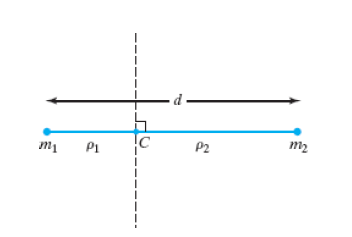
\includegraphics[width=0.4\textwidth]{Figures/6.2.png}
        \caption{
            \centering\parbox{\linewidth}{
                \centering
                用于计算双粒子刚性转子 \\
                转动惯量的轴线(虚线)。\\
                $C$是质心。
            }
        }
        \label{fig:6.2}
    \end{figure}
    转子绕我们选择的轴旋转的转动惯量为
    \begin{equation}
        I = m_1\rho_1^2 + m_2\rho_2^2
        \label{eq:6.50}
    \end{equation}
    使用式(\ref{eq:6.49}),我们可以将(\ref{eq:6.50})写成(问题6.14)
    \begin{equation}
        \boxed{
            I = \mu d^2
        }
        \label{eq:6.51}
    \end{equation}
    其中$\mu \equiv m_1m_2/(m_1+m_2)$是系统的折合质量,$d \equiv \rho_1 + \rho_2$是$m_1$和$m_2$之间的距离。双粒子刚性转子允许的能级由式(\ref{eq:6.47})给出:
    \begin{equation}
        \boxed{
            E = \frac{J\left(J+1\right)\hbar^2}{2I}, \quad J = 0, 1, 2, \ldots
        }
        \label{eq:6.52}
    \end{equation}
    最低的能级满足$E=0$,所以没有零点转动能。转动能为零,因此转子的角动量为零,这并不违反不确定性原理;回顾公式(\ref{eq:5.105})后面的讨论。请注意:$E$随着$J^2+J$的增大而增大,因此相邻旋转能级的间隔随着$J$的增大而增大。

    转子的能级(\ref{eq:6.52})是简并的吗?能量只取决于$J$,而波函数(\ref{eq:6.46})同时取决于$J$和$m$,其中$m\hbar$是转子角动量在$z$方向上的分量。对于每个$J$的值,都有$2J+1$个$m$的可能值,从$-J$到$J$。因此,能级是$\left(2J+1\right)$-重简并的。简并能级的状态具有不同的转子绕空间固定轴方向的角动量矢量方向。

    波函数(\ref{eq:6.46})中的$\theta$和$\phi$角是两个质点的相对坐标。如果我们建立一个笛卡尔坐标系,令转子的质心与原点重合,那么$\theta$和$\phi$将如图\ref{fig:6.3}所示。该坐标系与转子质心的平移运动相同,但不在空间中转动。

    转动角动量$\left[J\left(J+1\right)\hbar^2\right]^{1/2}$是两个粒子相对于系统质心$C$处原点的角动量。

    双原子分子的旋转能级可以用双粒子刚性转子模型(\ref{eq:6.52})来很好地近似。研究发现(\textit{Levine, Molecular Spectroscopy}, Section 4.4 ):当双原子分子吸收或发射辐射时,允许的纯转动跃迁由以下选律给出:
    \begin{equation}
        \Delta J = \pm 1
        \label{eq:6.53}
    \end{equation}
    此外,分子必须具有非零偶极矩,才能显示出纯转动光谱。\textit{纯转动跃迁}(pure rotational transition)是指只有转动量子数发生变化的跃迁。[振动-转动跃迁(第\ref{sec:4.3 Vibrations of Diatomic Molecules}节)涉及振动量子数和转动量子数的变化。]相邻较低旋转能级之间的能级间隔明显小于振动能级之间的能级间隔,纯转动光谱位于微波(或远红外)区域。因此,双原子分子纯转动光谱线的频率(近似值)为:
    \begin{equation}
        \nu = \frac{E_{J+1} - E_J}{h} = \frac{\left[\left(J+1\right)\left(J+2\right) - J\left(J+1\right)\right]\hbar^2}{8\pi^2 I} = 2\left(J+1\right)B
        \label{eq:6.54}
    \end{equation}
    \begin{equation}
        B \equiv h/8\pi^2 I, \quad J = 0, 1, 2, \ldots
        \label{eq:6.55}
    \end{equation}
    $B$称为分子的\textbf{转动常数}(rotational constant)。
    \begin{figure}[h!]
        \centering
        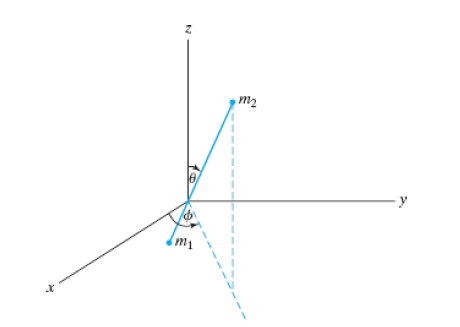
\includegraphics[width=0.4\textwidth]{Figures/6.3.png}
        \caption{双粒子刚性转子的坐标系}
        \label{fig:6.3}
    \end{figure}

    在室温下,具有较低$J$值的双粒子旋转能级间隔通常小于$kT$或与$kT$处于同一数量级,因此,玻尔兹曼分布律(\ref{eq:4.63})表明:室温下许多转动能级可以被显著占据。$J=0$的双原子分子吸收辐射后会产生一条频率为$2B$的谱线(对应$J = 0 \to 1$的跃迁),$J=1$的分子吸收辐射后会产生一条频率为$4B$的谱线(对应$J = 1 \to 2$的跃迁),$J=2$的分子吸收辐射后会产生一条频率为$6B$的谱线(对应$J = 2 \to 3$的跃迁),依此类推。见图\ref{fig:6.4}。
    \begin{figure}[h!]
        \centering
        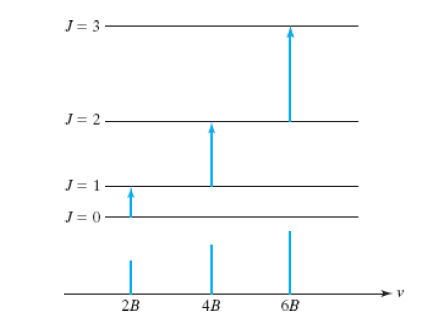
\includegraphics[width=0.4\textwidth]{Figures/6.4.png}
        \caption{双粒子刚性转子吸收跃迁}
        \label{fig:6.4}
    \end{figure}

    通过测量转动吸收频率可以得到$B$的值。根据$B$,我们可以得到分子的转动惯量$I$,根据$I$我们可以得到键长$d$。找到的$d$值是$v=0$振动运动的平均值。由于图4.6和图13.1中的势能曲线不对称,$d$比图13.1中的平衡键长略长。
    % 此处记得改引用!!!!!

    如第\ref{sec:4.3 Vibrations of Diatomic Molecules}节所述,$^1\mathrm{H}^{35}\mathrm{Cl}$和$^1\mathrm{H}^{37}\mathrm{Cl}$等同位素分子的电子能量曲线$U\left(R\right)$几乎相同,因此其平衡核间距也几乎相同。然而,不同的同位素质量会产生不同的转动惯量,从而产生不同的转动吸收频率。

    由于分子不是刚性的,因此双原子分子的旋转能级与刚性转子的旋转能级略有不同。由式(\ref{eq:6.52})和(\ref{eq:6.55}),双粒子刚性转子的能级为$E_{rot} = BhJ\left(J+1\right)$。由于分子振动的非谐性(图\ref{fig:4.6}、\ref{fig:4.5}),当振动量子数$v$增加时,核间距平均值也会增加,所以$v$增加时,转动惯量$I$也会增加,则转动常数$B$减小。为了考虑$B$对$v$的依赖性,在$E_{rot}$中用$B_v$代替$B$。振动能级$v$的\textit{平均转动常数}(mean rotational constant)$B_v$满足$B_v = B_e - \alpha_e\left(v+1/2\right)$,其中$B_e$是利用图\ref{fig:4.5}和\ref{fig:4.5}势能曲线底部的平衡核间距$R_e$计算得出的,\textit{振转耦合常数}(vibrational-rotational coupling constant)$\alpha_e$是一个大于零的常数(因分子的不同而异),且远小于$B_e$。此外,随着转动能量的增加,平衡核间距有非常轻微的增加[这种现象称为\textit{离心形变}(centrifugal distortion)]。这就在$E_{rot}$中引入了一项$-hDJ^2\left(J+1\right)^2$,其中离心形变常数$D$是一个极小的正常数,随着分子的不同而异。例如,对$^{12}\mathrm{C}^{15}\mathrm{O}$分子,$B_0 = 57636 \: \mathrm{MHz}$,$\alpha_e = 540 \: \mathrm{MHz}$,$D = 0.18 \: \mathrm{MHz}$。如第\ref{sec:4.3 Vibrations of Diatomic Molecules}节所述,对于轻双原子分子,几乎所有分子在室温下都处在基态振动能级,观测到的转动常数为$B_0$。

    有关双原子分子核运动的更多讨论,请参见第\ref{sec:13.2 Nuclear Motion in Diatomic Molecules}节。关于多原子分子的转动能,请参见\textit{Townes and Schawlow}, chaps. 2-4。

    \begin{examplebox}
        \textbf{例题:}分子$^{12}\mathrm{C}^{32}\mathrm{S}$的最低频率纯转动吸收线位于$48991.0 \: \mathrm{MHz}$。计算分子的键长。
        \\
        \\
        最低频率的转动吸收为$J = 0 \to 1$线。根据式(\ref{eq:1.4 Higher state to lower state delta energy})、(\ref{eq:6.52})和(\ref{eq:6.51}),有
        \begin{equation*}
            h\nu = E_{upper} - E_{lower} = \frac{1\left(2\right)\hbar^2}{2\mu d^2} - \frac{0\left(1\right)\hbar^2}{2\mu d^2}
        \end{equation*}
        其中$d = \left(h/4\pi^2\nu\mu\right)^{1/2}$。使用附录中的表A.3,有
        \begin{equation*}
            \mu = \frac{m_1m_2}{m_1 + m_2} = \frac{12\left(31.97207\right)}{\left(12+31.97207\right)}\frac{1}{6.02214\times 10^{23}} \: \mathrm{g} = 1.44885 \times 10^{-23} \: \mathrm{kg}
        \end{equation*}
        质量的国际单位为千克,则
        \begin{equation*}
            \begin{aligned}
                d = \frac{1}{2\pi}\left(\frac{h}{\nu_{0 \to 1}\mu}\right)^{1/2} & = \frac{1}{2\pi}\left[\frac{6.62607 \times 10^{-34} \: \mathrm{J \cdot s}}{\left(48991.0 \times 10^6\: \mathrm{s}^{-1}\right) \left(1.44885 \times 10^{-26} \: \mathrm{kg}\right)}\right]^{1/2} \\
                & = 1.5377 \times 10^{-10} \: \mathrm{m} = 1.5377 \: \mathrm{Å}
            \end{aligned}
        \end{equation*}
        \\
        \\
        \textbf{练习:}分子$^{12}\mathrm{C}^{16}\mathrm{O}$的$J = 1 \to 2$的纯转动跃迁位于$230.538 \: \mathrm{GHz}$。(1 GHz = $10^9$ Hz。)计算分子的键长。(\textit{答案:}$1.1309 \times 10^{-10} \: \mathrm{m}$。)
    \end{examplebox}

\section{氢原子}
\label{sec:6.5 The Hydrogen Atom}









\section{束缚态氢原子波函数}
\label{sec:6.6 The Bound-State Hydrogen-Atom Wave Functions}

\section{类氢轨道}
\label{sec:6.7 Hydrogenlike orbitals}

\section{塞曼效应}
\label{sec:6.8 Zeeman effect}

\section{径向薛定谔方程的数值解法}
\label{sec:6.9 Numerical Solution of the Radial Schrödinger Equation}

\section*{总结}

\section*{习题}
